% ============================================================================
% Fichier  : partie1/P01_C05_gestion_des_risques.tex
% Titre    : Gérer les Risques des Systèmes d'Information
% Auteur   : MINKA MI NGUIDJOÏ Thierry Emmanuel
% Version  : 1.0 -- novembre 2026
% ============================================================================
% Base : ACSI C03 (cartographie des risques résiduels de LiZbiZ, registre,
% options de traitement, SANAGA deux échelles).
% Sources : ISO 31000:2018 (processus) ; ISO/IEC 27005 (éditions 2018 et
% 2022) ; ANSSI, EBIOS Risk Manager (2018), cinq ateliers ; CLUSIF, MEHARI
% 2010 ; SEI, OCTAVE Allegro (2007) ; Freund et Jones (2014), FAIR ;
% COSO ERM 2004 et 2017.
% Simulation FAIR de R8 : script scratchpad fair_r8.py, graine 2026,
% 10 000 tirages : moyenne 87,2 M, médiane 0, P90 417 M, P95 582 M,
% P(perte > 0) 0,176, P(> 500 M) 0,073 ; après contrôle moyenne 12,4 M.
% Corrigés : corriges/Corr_C05.tex.
% ============================================================================

\chapter{Gérer les Risques des Systèmes d'Information}
\label{chap:gestion-risques}
\chaptermark{Gérer les risques}

\epigraph{%
    « Une méthode d'analyse de risques ne dit pas ce qui va arriver.\\
    Elle oblige à dire ce que l'on sait, et ce que l'on ignore. »%
}{Principe du gestionnaire de risques}

\niveauChapitre{Fondamental à intermédiaire}{%
    Maîtrise du Chapitre~\ref{chap:risque} (notions, échelle, mesure
    quantitative)%
}

\begin{boxobjectifs}
\begin{itemize}
    \item Décrire le processus de management des risques de l'ISO~31000 et
          son application à la sécurité de l'information (ISO/IEC~27005).
    \item Construire une cartographie des risques et en déduire les
          priorités de traitement.
    \item Choisir et documenter une option de traitement~; rédiger un plan
          de traitement et des indicateurs de risque.
    \item Conduire les cinq ateliers de la méthode EBIOS Risk Manager sur un
          cas.
    \item Situer MEHARI et OCTAVE Allegro, et dire quand les utiliser.
    \item Réaliser une analyse FAIR par simulation de Monte-Carlo, et lire
          la distribution de pertes obtenue.
    \item Auditer le dispositif de gestion des risques d'une organisation.
\end{itemize}
\end{boxobjectifs}

\bigskip

% ============================================================================
\section*{Question directrice : comment passer d'une liste à une décision~?}
% ============================================================================

Mme~NKENG dispose désormais d'un registre de huit risques cotés
(Chapitre~\ref{chap:risque}). Le conseil d'administration de LiZbiZ lui pose
trois questions~: «~Que faisons-nous en premier~? Combien cela coûte-t-il~?
Comment saurons-nous que cela marche~?~» Un registre ne répond à aucune des
trois. Il faut un processus, qui relie l'appréciation des risques à leur
traitement et à leur suivi, et des méthodes, qui structurent l'analyse.

\medskip
\textbf{Plan du chapitre.}
\begin{enumerate}
    \item Le processus de management des risques
          (section~\ref{sec:c05-processus}).
    \item La cartographie et le traitement
          (section~\ref{sec:c05-carto}).
    \item La méthode EBIOS Risk Manager (section~\ref{sec:c05-ebios}).
    \item MEHARI et OCTAVE Allegro (section~\ref{sec:c05-autres}).
    \item La méthode FAIR et la simulation (section~\ref{sec:c05-fair}).
    \item Auditer la gestion des risques (section~\ref{sec:c05-auditer}).
\end{enumerate}

\separateur

% ============================================================================
\section{Le Processus de Management des Risques}
\label{sec:c05-processus}
% ============================================================================

\subsection{Le processus de l'ISO 31000}

L'ISO~31000:2018 décrit un processus en boucle, applicable à tout
risque~\cite{iso31000_2018}.

\begin{enumerate}
    \item \textbf{Établir le contexte}~: périmètre, objectifs, critères de
          risque (échelles, appétence).
    \item \textbf{Apprécier les risques}, en trois temps~:
          \emph{identifier} (quels risques~?), \emph{analyser} (quelle
          probabilité, quel impact~?), \emph{évaluer} (comparer à
          l'appétence, décider des priorités).
    \item \textbf{Traiter}~: choisir une option et la mettre en œuvre.
    \item \textbf{Surveiller et revoir}~: suivre les risques, les
          traitements, les indicateurs.
    \item \textbf{Communiquer et consulter}, à toutes les étapes.
    \item \textbf{Enregistrer et rendre compte}~: documenter les décisions.
\end{enumerate}

\noindent\begin{minipage}{\linewidth}
\begin{center}
\begin{tikzpicture}[
    etape/.style={draw=CouleurPrimaire, fill=CouleurPrimaire!8, rounded corners,
                  minimum width=3.2cm, minimum height=0.8cm, font=\small, align=center},
    fleche/.style={-{Stealth}, thick, CouleurPrimaire}]
\node[etape] (c) at (0,3) {Contexte et critères};
\node[etape] (a) at (0,1.8) {Appréciation\\ \footnotesize identifier, analyser, évaluer};
\node[etape] (t) at (0,0.5) {Traitement};
\node[etape] (s) at (0,-0.7) {Surveillance et revue};
\node[etape, minimum height=4.4cm, minimum width=2.4cm] (com) at (-3.6,1.15)
     {Communication\\ et\\ consultation};
\node[etape, minimum height=4.4cm, minimum width=2.4cm] (enr) at (3.6,1.15)
     {Enregistrement\\ et\\ compte rendu};
\draw[fleche] (c) -- (a);
\draw[fleche] (a) -- (t);
\draw[fleche] (t) -- (s);
\draw[fleche] (s.east) -- ++(0.5,0) |- (c.east);
\end{tikzpicture}
\end{center}
\vspace{-0.4em}
\begin{center}{\small\itshape Figure~5.1. Le processus de management des
risques (d'après l'ISO~31000:2018)}\end{center}
\end{minipage}

\subsection{La sécurité de l'information~: ISO/IEC 27005}

L'ISO/IEC~27005 applique ce processus aux risques de sécurité de
l'information, au service du système de management de la sécurité de
l'ISO/IEC~27001 (Chapitre~\ref{chap:audit-smsi}). L'édition de 2018,
présente dans le dossier \texttt{Normes}~\cite{iso27005_2018}, a été
remplacée par celle de 2022~\cite{iso27005_2022}, qui admet deux manières
d'identifier les risques~: à partir des événements et de leurs
conséquences, ou à partir des actifs, des menaces et des vulnérabilités.

\begin{boxinfo}
\textbf{Vérifier l'édition.} Un rapport d'audit cite toujours l'édition de
la norme appliquée. Une organisation dont la procédure renvoie à
l'édition de 2018 n'est pas en faute pour autant~; elle doit seulement
avoir décidé, en connaissance de cause, de la conserver ou de migrer.
\end{boxinfo}

\subsection{Le management des risques de l'entreprise~: COSO ERM}

Le COSO~ERM étend le contrôle interne à la gestion des risques de toute
l'entreprise. Sa version de 2004 compte huit éléments, de l'environnement
interne au pilotage~\cite{coso2004ermfr}~; celle de 2017 en retient cinq
composantes et intègre le risque à la stratégie et à la
performance~\cite{coso2017erm}. Pour l'auditeur des SI, l'apport principal
est l'exigence que le risque informatique soit apprécié \emph{avec} les
autres risques de l'entreprise, sur la même échelle.

% ============================================================================
\section{Cartographier et Traiter}
\label{sec:c05-carto}
% ============================================================================

\subsection{La matrice probabilité × impact}

La \termecle{cartographie des risques}\index{cartographie des risques}
représente chaque risque par sa position dans une matrice probabilité ×
impact. Les zones de couleur traduisent l'appétence~: rouge, intolérable~;
orange, à traiter~; vert, accepté.

\noindent\begin{minipage}{\linewidth}
\begin{center}
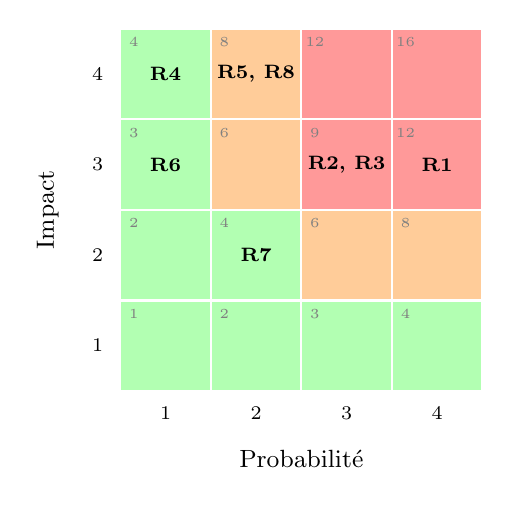
\begin{tikzpicture}[scale=1.15]
\foreach \p in {1,...,4}{
    \foreach \i in {1,...,4}{
        \pgfmathtruncatemacro{\s}{\p*\i}
        \ifnum\s>8 \def\coul{red!40}\else\ifnum\s>4 \def\coul{orange!40}\else\def\coul{green!30}\fi\fi
        \fill[\coul] (\p-1,\i-1) rectangle (\p,\i);
        \draw[white, thick] (\p-1,\i-1) rectangle (\p,\i);
        \node[font=\tiny, color=gray] at (\p-0.85,\i-0.15) {\s};
    }
}
\node[font=\scriptsize\bfseries] at (3.5,2.5) {R1};
\node[font=\scriptsize\bfseries] at (2.5,2.5) {R2, R3};
\node[font=\scriptsize\bfseries] at (1.5,3.5) {R5, R8};
\node[font=\scriptsize\bfseries] at (0.5,3.5) {R4};
\node[font=\scriptsize\bfseries] at (0.5,2.5) {R6};
\node[font=\scriptsize\bfseries] at (1.5,1.5) {R7};
\foreach \k in {1,...,4}{
    \node[font=\scriptsize] at (\k-0.5,-0.25) {\k};
    \node[font=\scriptsize] at (-0.25,\k-0.5) {\k};
}
\node[font=\small] at (2,-0.75) {Probabilité};
\node[font=\small, rotate=90] at (-0.8,2) {Impact};
\end{tikzpicture}
\end{center}
\vspace{-0.4em}
\begin{center}{\small\itshape Figure~5.2. Cartographie des risques
résiduels de LiZbiZ}\end{center}
\end{minipage}

\medskip

La cartographie se lit en trois temps~: les risques en zone rouge sont
traités en priorité~; les risques d'impact~4 restent sous surveillance même
en zone verte, car une erreur sur leur probabilité serait coûteuse~; et
l'écart entre risque inhérent et risque résiduel montre ce que les
contrôles apportent réellement.

\subsection{Quatre options de traitement}

\begin{tableaucours}{L{2.4cm}L{5.0cm}L{4.8cm}}{%
    \tableauHeader{Option} &
    \tableauHeader{Principe} &
    \tableauHeader{Exemple chez LiZbiZ}
}
Réduire & Ajouter ou renforcer des contrôles & Séparer réception et
ajustement (R1) \\
Transférer & Assurance, sous-traitance, sans transférer la responsabilité
& Police d'assurance cyber pour R8 \\
Éviter & Renoncer à l'activité qui crée le risque & Cesser la saisie des
paiements hors application \\
Accepter & Dans les limites de l'appétence, par une décision écrite & R6
résiduel~3, accepté par le comité de direction \\
\end{tableaucours}
\vspace{-0.8em}
\begin{center}{\small\itshape Tableau~5.1. Les options de
traitement}\end{center}

\begin{boxalert}
\textbf{Violation typique.} Considérer qu'un risque confié à un prestataire
« n'est plus le nôtre ».

\smallskip
\textbf{Règle~:} on transfère une conséquence financière (assurance) ou une
exécution (sous-traitance), jamais la responsabilité. Le donneur d'ordre
reste comptable devant ses clients, ses régulateurs et la loi
(Chapitre~\ref{chap:audit-tiers}).
\end{boxalert}

\subsection{Le plan de traitement}

\begin{boxprocedure}
\textbf{Le registre et le plan de traitement.} Pour qu'un auditeur puisse
s'appuyer sur la gestion des risques, chaque risque traité indique~:
\begin{itemize}
    \item le risque, l'objectif menacé et son propriétaire~;
    \item la cotation inhérente, avec la justification de la probabilité et
          de l'impact~;
    \item les contrôles qui le réduisent, avec la date et le résultat de leur
          dernier test~;
    \item la cotation résiduelle et la décision de traitement~;
    \item les actions du plan, leur responsable, leur échéance et leur
          coût~;
    \item la cotation cible attendue après les actions~;
    \item pour un risque accepté, la décision écrite de l'instance
          compétente.
\end{itemize}
\end{boxprocedure}

\begin{tableaucours}{cL{4.2cm}L{2.6cm}L{1.8cm}cc}{%
    \tableauHeader{Réf.} &
    \tableauHeader{Action} &
    \tableauHeader{Responsable} &
    \tableauHeader{Échéance} &
    \tableauHeader{Rés.} & \tableauHeader{Cible}
}
R1 & Retirer F4 aux magasiniers~; validation au-delà de 500~000 & DAF &
30/06/2026 & 12 & 6 \\
R2 & Validation des créations de fournisseurs par le DAF & DAF &
30/06/2026 & 9 & 6 \\
R3 & Procédure de départ, revue trimestrielle des comptes & Resp. RH et
resp. informatique & 31/05/2026 & 9 & 3 \\
R5 & Restauration de test mensuelle & Resp. informatique & 31/07/2026 & 8
& 4 \\
R8 & Sauvegardes hors ligne~; correctifs sous 30 jours & Resp.
informatique & 30/09/2026 & 8 & 4 \\
\end{tableaucours}
\vspace{-0.8em}
\begin{center}{\small\itshape Tableau~5.2. Plan de traitement de LiZbiZ
(extrait)}\end{center}

\subsection{Les indicateurs de risque}

\begin{boxdef}
\termecle{Indicateur clé de risque}\index{indicateur clé de risque}
(\textit{key risk indicator}, KRI)~: mesure régulière qui signale qu'un
risque augmente avant qu'il ne se réalise. Il porte sur une cause ou une
vulnérabilité, pas sur l'incident lui-même.
\end{boxdef}

\begin{tableaucours}{cL{5.2cm}L{3.0cm}L{2.8cm}}{%
    \tableauHeader{Réf.} &
    \tableauHeader{Indicateur} &
    \tableauHeader{Fréquence} &
    \tableauHeader{Seuil d'alerte}
}
R1 & Montant des ajustements négatifs du mois, par entrepôt & Mensuelle &
plus de 10~millions \\
R3 & Comptes actifs d'agents partis depuis plus de 48~h & Hebdomadaire &
plus de 0 \\
R5 & Jours depuis la dernière restauration réussie & Quotidienne & plus de
35 \\
R8 & Serveurs avec un correctif critique de plus de 30~jours &
Hebdomadaire & plus de 0 \\
\end{tableaucours}
\vspace{-0.8em}
\begin{center}{\small\itshape Tableau~5.3. Indicateurs clés de risque de
LiZbiZ}\end{center}

\begin{boxscenario}{Opération SANAGA. Deux registres, deux échelles}
\textbf{Constatation.} La BANQUE SANAGA tient un registre des risques de
crédit et de marché, coté de 1 à 4, et la DSI un registre des risques
informatiques, coté de 1 à 5 avec d'autres critères d'impact.

\medskip
\textbf{Analyse} (confiance élevée). Le conseil ne peut pas comparer un
risque informatique à un risque de crédit, donc ne peut pas arbitrer. La
panne de mars~2026, cotée « 3 sur 5 » par la DSI, n'est jamais apparue
parmi les risques majeurs de la banque. Règle~: le risque informatique est
un risque de l'entreprise, à coter sur l'échelle commune.
\end{boxscenario}

% ============================================================================
\section{La Méthode EBIOS Risk Manager}
\label{sec:c05-ebios}
% ============================================================================

\subsection{Présentation}

EBIOS Risk Manager est la méthode d'appréciation et de traitement des
risques numériques publiée par l'Agence nationale de la sécurité des
systèmes d'information (ANSSI, France) en 2018~\cite{anssi2018ebios}. Elle
part des missions de l'organisation et de ce qu'un attaquant peut viser,
plutôt que d'un inventaire de vulnérabilités. Elle s'organise en cinq
ateliers, et en deux cycles~: un cycle stratégique, revu tous les trois ans
environ, et un cycle opérationnel, revu chaque année.

\begin{tableaucours}{cL{3.4cm}L{4.4cm}L{3.6cm}}{%
    \tableauHeader{N°} &
    \tableauHeader{Atelier} &
    \tableauHeader{Question} &
    \tableauHeader{Produit}
}
1 & Cadrage et socle de sécurité & Que protège-t-on, et à quelles règles
l'organisation est-elle déjà tenue~? & Valeurs métier, biens supports,
événements redoutés, écarts au socle \\
2 & Sources de risque & Qui pourrait attaquer, et dans quel but~? &
Couples source de risque et objectif visé, retenus \\
3 & Scénarios stratégiques & Par quel chemin, à travers l'écosystème~? &
Cartographie des parties prenantes, scénarios stratégiques \\
4 & Scénarios opérationnels & Par quels modes opératoires techniques~? &
Scénarios opérationnels et leur vraisemblance \\
5 & Traitement du risque & Que fait-on, et que reste-t-il~? & Stratégie de
traitement, plan d'amélioration, risques résiduels \\
\end{tableaucours}
\vspace{-0.8em}
\begin{center}{\small\itshape Tableau~5.4. Les cinq ateliers d'EBIOS Risk
Manager}\end{center}

\subsection{Les ateliers appliqués à LiZbiZ}

\begin{boxscenario}{Opération LIZBIZ. Atelier 1, cadrage}
\textbf{Mission retenue.} Livrer et facturer les clients dans les délais.

\textbf{Valeurs métier.} VM1 le suivi des expéditions~; VM2 la facturation~;
VM3 les paiements aux fournisseurs.

\textbf{Biens supports.} L'application intégrée, les quatre centres de
données (Douala, Yaoundé, Garoua, Bafoussam), le réseau entre les sites,
la messagerie.

\textbf{Événements redoutés.} ER1 indisponibilité de la facturation plus de
3~jours (gravité critique)~; ER2 paiements frauduleux (gravité majeure)~;
ER3 divulgation des données clients (gravité majeure, loi n°~2024/017).

\textbf{Socle.} Écarts relevés à la loi n°~2010/012 (sécurité des
systèmes) et à la politique de sécurité interne, inexistante.
\end{boxscenario}

\begin{boxscenario}{Opération LIZBIZ. Atelier 2, sources de risque}
\begin{tableaucours}{L{3.6cm}L{4.4cm}c}{%
    \tableauHeader{Source de risque} &
    \tableauHeader{Objectif visé} &
    \tableauHeader{Retenu}
}
Groupe cybercriminel & Rançon (chiffrement des serveurs) & Oui \\
Salarié ou complice interne & Détournement de fonds par fournisseur fictif
& Oui \\
Ancien salarié & Revente de données clients & Oui \\
Concurrent & Espionnage des tarifs & Non (motivation faible, ressources
faibles) \\
\end{tableaucours}
\end{boxscenario}

\begin{boxscenario}{Opération LIZBIZ. Ateliers 3 et 4, un scénario}
\textbf{Scénario stratégique.} Un groupe cybercriminel compromet le
prestataire de maintenance de Garoua, qui dispose d'un accès distant, puis
chiffre les serveurs de facturation (vise ER1).

\textbf{Scénario opérationnel.} Hameçonnage d'un technicien du prestataire~;
réutilisation de son accès distant sans double authentification~;
élévation de privilèges sur un serveur non corrigé~; désactivation des
sauvegardes accessibles en réseau~; chiffrement.

\textbf{Vraisemblance.} Élevée~: chaque étape repose sur une vulnérabilité
constatée (accès distant à facteur unique, correctifs irréguliers,
sauvegardes en ligne).
\end{boxscenario}

\begin{boxscenario}{Opération LIZBIZ. Atelier 5, traitement}
\textbf{Mesures retenues.} Double authentification pour tout accès
distant~; clause de sécurité et droit d'audit dans le contrat du
prestataire~; correctifs critiques sous 30~jours~; sauvegardes hors ligne
testées chaque mois.

\textbf{Risque résiduel.} ER1 passe de gravité critique et vraisemblance
élevée à gravité critique et vraisemblance faible~: la gravité ne baisse
pas (une indisponibilité reste critique), seule la vraisemblance baisse.
Le risque résiduel est accepté par le comité de direction, avec suivi des
indicateurs R5 et R8 du Tableau~5.3.
\end{boxscenario}

\begin{boxinfo}
\textbf{Ce qu'apporte EBIOS par rapport au registre.} Le registre de
Mme~NKENG cotait R8 (rançongiciel) à partir d'un jugement global. EBIOS
oblige à écrire le chemin d'attaque, étape par étape~; chaque étape est une
hypothèse vérifiable par l'auditeur (l'accès distant est-il à facteur
unique~? les sauvegardes sont-elles en ligne~?). Une cotation devient une
liste de faits à vérifier.
\end{boxinfo}

% ============================================================================
\section{MEHARI et OCTAVE Allegro}
\label{sec:c05-autres}
% ============================================================================

\subsection{MEHARI}

MEHARI (\textit{Méthode harmonisée d'analyse de risques}) est publiée par
le Club de la sécurité de l'information français
(CLUSIF)~\cite{clusif2010mehari}. Elle repose sur des bases de
connaissances~: une liste de scénarios de risque types, et des
questionnaires d'audit des services de sécurité qui mesurent la qualité des
mesures en place. La gravité d'un scénario se déduit de sa potentialité et
de son impact, chacun modulé par la qualité mesurée des services de
sécurité.

\subsection{OCTAVE Allegro}

OCTAVE Allegro est une méthode allégée publiée par le Software Engineering
Institute de l'université Carnegie Mellon~\cite{caralli2007octave}. Elle
est centrée sur les actifs informationnels et leurs « conteneurs »
(techniques, physiques, humains), et conçue pour être menée par une petite
équipe interne en quelques ateliers.

\subsection{Choisir une méthode}

\begin{tableaucours}{L{2.6cm}L{3.6cm}L{3.0cm}L{3.0cm}}{%
    \tableauHeader{Méthode} &
    \tableauHeader{Point de départ} &
    \tableauHeader{Résultat} &
    \tableauHeader{Adaptée à}
}
EBIOS RM & Missions et scénarios d'attaque & Scénarios, plan de traitement
& Organisation exposée à des attaquants ciblés \\
MEHARI & Bases de scénarios et questionnaires & Gravité par scénario,
qualité des mesures & Organisation qui veut un diagnostic complet et
outillé \\
OCTAVE Allegro & Actifs informationnels & Risques par actif & Petite
équipe, première analyse \\
FAIR & Un scénario de perte & Distribution de pertes en valeur & Décision
d'investissement \\
\end{tableaucours}
\vspace{-0.8em}
\begin{center}{\small\itshape Tableau~5.5. Quatre méthodes et leurs
usages}\end{center}

Les méthodes se combinent~: EBIOS ou OCTAVE identifient et structurent les
scénarios, FAIR chiffre ceux qui demandent un arbitrage budgétaire.

% ============================================================================
\section{La Méthode FAIR et la Simulation}
\label{sec:c05-fair}
% ============================================================================

\subsection{La décomposition FAIR}

FAIR (\textit{Factor Analysis of Information Risk}) décompose le risque en
facteurs estimables~\cite{freund2014fair}.

\begin{boxdef}
\termecle{Fréquence des événements de perte}\index{FAIR} (LEF)~: nombre
d'événements de perte par an. $\text{LEF} = \text{TEF} \times V$, où TEF
est la fréquence des tentatives (\textit{threat event frequency}) et $V$ la
vulnérabilité, probabilité qu'une tentative réussisse.

\medskip
\termecle{Ampleur de la perte} (LM)~: perte causée par un événement,
primaire (arrêt, reconstitution, rançon) et secondaire (amendes,
réputation, contentieux).

\medskip
\textbf{Risque}~: distribution de la perte annuelle, résultant de LEF et
LM.
\end{boxdef}

\subsection{Estimer chaque facteur par un intervalle}

\begin{boxscenario}{Opération LIZBIZ. R8 en facteurs}
\textbf{Estimations} (DSI et AUDIX CONSEIL, intervalles à 90~\%, valeur la
plus probable entre parenthèses)~:
\begin{itemize}
    \item TEF~: de 0,5 à 6 tentatives sérieuses par an (2)~;
    \item $V$~: de 2 à 15~\% (5~\%), compte tenu de l'accès distant à
          facteur unique et des correctifs irréguliers~;
    \item LM~: de 100 à 900~millions FCFA par événement (300), arrêt de la
          facturation et reconstitution comprises.
\end{itemize}
\end{boxscenario}

\subsection{Simuler}

Multiplier les valeurs les plus probables ($2 \times 0{,}05 \times 300 =
30$~millions par an) donne un chiffre trompeur~: il ignore l'étendue des
intervalles et l'asymétrie des pertes. La simulation de Monte-Carlo tire
au hasard, des milliers de fois, une valeur de chaque facteur dans sa
distribution, et en déduit la distribution de la perte annuelle.

\begin{boxoutils}{Simulation FAIR en Python}
\begin{lstlisting}[language=Python]
import math, random
random.seed(2026)                   # reproductibilité du résultat
N, pertes = 10_000, []
for _ in range(N):
    tef = random.triangular(0.5, 6.0, 2.0)    # tentatives par an
    v   = random.triangular(0.02, 0.15, 0.05) # succès d'une tentative
    lef = tef * v                             # événements par an
    k, p, seuil = 0, 1.0, math.exp(-lef)      # tirage de Poisson
    while True:
        p *= random.random()
        if p <= seuil: break
        k += 1
    pertes.append(sum(random.triangular(100, 900, 300)
                      for _ in range(k)))     # millions FCFA
pertes.sort()
print(sum(pertes) / N, pertes[N // 2], pertes[int(0.9 * N)])
\end{lstlisting}
\end{boxoutils}

\begin{boxlecture}{Résultat de la simulation de R8}
Sur 10~000~années simulées (graine 2026)~:
\begin{itemize}
    \item perte annuelle moyenne~: environ 87~millions FCFA~;
    \item médiane~: 0 (plus d'une année sur deux sans événement)~;
    \item probabilité d'au moins un événement dans l'année~: 17,6~\%~;
    \item 90\textsuperscript{e} centile~: environ 417~millions~;
          95\textsuperscript{e}~: environ 582~millions~;
    \item probabilité de perdre plus de 500~millions dans l'année~: 7,3~\%.
\end{itemize}

\textbf{Analyse.} La moyenne (87~millions) est presque trois fois le
« calcul rapide » de 30~millions, à cause de l'asymétrie des pertes. Le
conseil peut désormais raisonner en probabilité de dépassement~: une
année sur quatorze environ, LiZbiZ perdrait plus de 500~millions. Avec les
mesures de l'atelier~5 (vulnérabilité ramenée à 1 à 6~\%, perte à 40 à
300~millions), la même simulation donne une moyenne d'environ
12~millions et une probabilité de dépasser 500~millions pratiquement nulle.
\end{boxlecture}

\noindent\begin{minipage}{\linewidth}
\begin{center}
\begin{tikzpicture}
\begin{axis}[width=11cm, height=5.2cm,
    xlabel={Perte annuelle $x$ (millions FCFA)},
    ylabel={$P(\text{perte} > x)$},
    xmin=0, xmax=900, ymin=0, ymax=0.2,
    yticklabel style={/pgf/number format/fixed},
    grid=major, grid style={gray!25}, font=\small]
\addplot[thick, CouleurAccent, mark=*, mark size=1.5pt]
    coordinates {(0,0.176) (200,0.166) (300,0.140) (417,0.100) (500,0.073) (582,0.050) (700,0.029) (900,0.011)};
\end{axis}
\end{tikzpicture}
\end{center}
\vspace{-0.4em}
\begin{center}{\small\itshape Figure~5.3. Courbe de dépassement de R8
(points issus de la simulation)}\end{center}
\end{minipage}

\begin{boxalert}
\textbf{Violation typique.} Présenter le résultat d'une simulation comme une
mesure, sans dire d'où viennent les intervalles.

\smallskip
\textbf{Règle~:} un résultat FAIR vaut ce que valent ses estimations. Le
rapport cite, pour chaque facteur, la source de l'intervalle (données
d'incidents, jugement d'expert calibré) et la graine de la simulation, pour
qu'un tiers puisse la refaire.
\end{boxalert}

% ============================================================================
\section{Auditer la Gestion des Risques}
\label{sec:c05-auditer}
% ============================================================================

L'auditeur n'a pas à refaire l'analyse de risques~: il juge si le dispositif
permet à la direction de connaître et de traiter ses risques.

\begin{boxobjet}{Le registre est justifié}
\textbf{Objectif.} Les priorités de traitement reposent sur des cotations
fondées.

\textbf{Critère.} Chaque risque de score résiduel supérieur ou égal à 9
porte une justification de la probabilité et de l'impact, et renvoie au
rapport de test des contrôles qui le réduisent (procédure de gestion des
risques, ISO~31000 § 6.4).

\textbf{Question.} Les risques intolérables du registre sont-ils justifiés
et leurs contrôles testés~?

\textbf{Risque.} La direction arbitre sur des cotes arbitraires~; un risque
majeur reste sous-estimé.

\textbf{Conséquence.} Ressources mal allouées~; incident non anticipé.

\textbf{Test.} Pour chaque risque intolérable, lecture de la justification
et du rapport de test~; recalcul du résiduel.

\textbf{Preuve et trace.} Copie du registre daté, rapports de test,
feuille de recalcul.
\end{boxobjet}

\begin{boxprocedure}
\textbf{Programme d'audit de la gestion des risques (extrait)}
\begin{enumerate}
    \item Obtenir la procédure, l'échelle, l'appétence approuvée et sa date.
    \item Vérifier que le périmètre couvre les risques informatiques, sur la
          même échelle que les autres risques.
    \item Pour un échantillon de risques, vérifier la justification, le
          propriétaire, le test des contrôles, la décision de traitement.
    \item Vérifier l'avancement du plan de traitement et le suivi des
          indicateurs.
    \item Vérifier qu'un risque accepté l'a été par l'instance compétente,
          par écrit.
    \item Vérifier la mise à jour après les incidents majeurs de la période.
\end{enumerate}
\end{boxprocedure}

\begin{boxmetier}{Gestionnaire de risques}
\textbf{Tenir une cartographie utile}
\begin{enumerate}
    \item Faire approuver l'échelle de cotation et l'appétence par le
          conseil, avant toute cotation.
    \item Désigner un propriétaire par risque, au niveau de la direction.
    \item Ne réduire le risque résiduel que sur la base de contrôles testés.
    \item Mettre à jour la cartographie au moins une fois par an, et après
          tout incident majeur.
    \item Présenter au comité d'audit les risques en zone rouge et les
          décisions d'acceptation.
\end{enumerate}
\end{boxmetier}

\begin{boxmetier}{RSSI}
\textbf{Alimenter EBIOS avec des faits.} Le RSSI fournit à chaque atelier
les éléments vérifiables~: état des correctifs, liste des accès distants,
résultat des tests de sauvegarde. Un scénario opérationnel qui repose sur
une hypothèse non vérifiée est marqué comme tel.
\end{boxmetier}

\begin{boxinfo}
\textbf{Ce que dit la recherche.} Une méthode d'analyse de risques produit
des cotes~; l'auditologie~\cite{minka2026auditologie} demande en plus ce que
l'on sait de chaque cote. Les intervalles de FAIR et les écarts entre
évaluateurs (Chapitre~\ref{chap:risque}) sont deux façons de rendre cette
connaissance visible, que la lecture $\mu$, $U$, $H$ rend comparable d'un
domaine à l'autre.
\end{boxinfo}

\separateur

\begin{boxresume}
\textbf{Ce qu'il faut retenir de ce chapitre~:}
\begin{itemize}
    \item \textbf{Le processus ISO~31000}~: contexte, appréciation
          (identifier, analyser, évaluer), traitement, surveillance, avec
          communication et enregistrement à chaque étape~; l'ISO/IEC~27005
          l'applique à la sécurité de l'information.
    \item \textbf{La cartographie} montre les priorités~; le plan de
          traitement les transforme en actions datées et chiffrées~; les
          indicateurs clés signalent un risque qui monte.
    \item \textbf{Quatre options}~: réduire, transférer, éviter, accepter~;
          la responsabilité ne se transfère pas.
    \item \textbf{EBIOS Risk Manager}~: cinq ateliers, du cadrage au
          traitement, qui transforment une cote en chemin d'attaque
          vérifiable.
    \item \textbf{MEHARI} et \textbf{OCTAVE Allegro} offrent un diagnostic
          outillé ou allégé~; \textbf{FAIR} chiffre un scénario en
          distribution de pertes par simulation.
    \item \textbf{Auditer la gestion des risques}, c'est vérifier les
          justifications, les tests, les décisions et le suivi, pas refaire
          l'analyse.
\end{itemize}
\end{boxresume}

\begin{boxinfo}
\textbf{Points de contrôle de l'élève.} Je sais~: dessiner le processus
ISO~31000~; nommer les cinq ateliers d'EBIOS~; écrire un indicateur clé de
risque~; décomposer un risque en facteurs FAIR~; lire une courbe de
dépassement~; rédiger trois étapes d'un programme d'audit de la gestion des
risques.
\end{boxinfo}

\bigskip

\begin{boxexo}[title={\ding{45}\quad Exercice~5.1. Le processus \niveaubase}]
Pour chacune des activités suivantes, indiquez l'étape du processus
ISO~31000 à laquelle elle appartient~: (a) le conseil fixe l'appétence~;
(b) trois responsables cotent R8~; (c) on compare R1 au seuil de 9~; (d) on
retire le droit F4 aux magasiniers~; (e) on suit chaque mois le montant des
ajustements négatifs.
\end{boxexo}

\begin{boxexo}[title={\ding{45}\quad Exercice~5.2. Choisir une option \niveaubase}]
Proposez une option de traitement, justifiée, pour R4, R6 et R7 du registre
de LiZbiZ.
\end{boxexo}

\begin{boxexo}[title={\ding{45}\quad Exercice~5.3. Des indicateurs \niveaumoyen}]
Proposez un indicateur clé de risque, sa fréquence et son seuil d'alerte
pour R2 et R6. Expliquez pourquoi « nombre d'incidents de fraude » n'est pas
un bon indicateur clé de risque.
\end{boxexo}

\begin{boxexo}[title={\ding{45}\quad Exercice~5.4. Atelier 2 d'EBIOS \niveaumoyen}]
Pour la BANQUE SANAGA, proposez quatre couples source de risque et
objectif visé, et dites lesquels vous retenez, en justifiant par la
motivation et les ressources de la source.
\end{boxexo}

\begin{boxexo}[title={\ding{45}\quad Exercice~5.5. Un scénario opérationnel \niveaumoyen}]
Rédigez, pour l'événement redouté ER2 de LiZbiZ (paiements frauduleux), un
scénario stratégique et le scénario opérationnel correspondant, en quatre
étapes. Pour chaque étape, indiquez le fait que l'auditeur devrait vérifier.
\end{boxexo}

\begin{boxexo}[title={\ding{45}\quad Exercice~5.6. Le calcul rapide \niveaumoyen}]
Expliquez pourquoi le produit des valeurs les plus probables
($2 \times 0{,}05 \times 300$) sous-estime la perte moyenne de R8. Calculez
la moyenne de chaque loi triangulaire (la moyenne de la loi triangulaire
de paramètres $a$, $b$, $c$ vaut $(a+b+c)/3$) et vérifiez que leur produit
est proche du résultat de la simulation.
\end{boxexo}

\begin{boxexo}[title={\ding{45}\quad Exercice~5.7. Lire une distribution \niveaumoyen}]
Le conseil de LiZbiZ envisage une assurance cyber qui couvre les pertes
au-delà de 200~millions par an, plafonnées à 1~milliard, pour une prime de
25~millions. À partir du résultat de la simulation, quelles informations
supplémentaires demandez-vous pour conseiller le conseil~? Quelle donnée
de la simulation est la plus utile ici~?
\end{boxexo}

\begin{boxexo}[title={\ding{45}\quad Exercice~5.8. Auditer un registre \niveaumoyen}]
Le registre de la BANQUE SANAGA contient 64~risques, dont 9 informatiques.
Rédigez une fiche d'assertion pour le contrôle « les risques informatiques
sont cotés sur l'échelle commune de la banque », puis cotez-la à partir de
la constatation du scénario « Deux registres, deux échelles ».
\end{boxexo}

\begin{boxexo}[title={\ding{45}\quad Exercice~5.9. Choisir une méthode \niveauexpert}]
L'agence publique ANPP veut analyser les risques de sa nouvelle plateforme
de paie, avec une équipe de trois personnes et sans budget de conseil. Le
ministère des Finances exige un chiffrage des pertes possibles avant de
financer un site de secours. Quelle combinaison de méthodes recommandez-
vous, et dans quel ordre~? Justifiez.
\end{boxexo}

\begin{boxexo}[title={\ding{45}\quad Exercice~5.10. Simulation et décision \niveauexpert}]
Modifiez la simulation de la section~\ref{sec:c05-fair} pour comparer deux
mesures~: (A) double authentification des accès distants, qui ramène $V$ à
1 à 6~\% (2~\%)~; (B) sauvegardes hors ligne testées, qui ramènent la perte
par événement à 40 à 300~millions (100). Écrivez le code, décrivez le
résultat attendu (sans l'exécuter, en raisonnant sur les moyennes), et
dites quelle mesure vous recommanderiez si une seule était finançable.
\end{boxexo}

\bigskip

\begin{boxinfo}
\textbf{Pour aller plus loin.}
\begin{itemize}
    \item ANSSI, \textit{EBIOS Risk Manager. Le guide}~\cite{anssi2018ebios}~:
          la méthode complète, avec un cas d'étude.
    \item J.~Freund et J.~Jones, \textit{Measuring and Managing
          Information Risk: A FAIR Approach}~\cite{freund2014fair}~: la
          référence de la méthode FAIR.
    \item ISO/IEC~27005:2022~\cite{iso27005_2022}~: le processus appliqué à
          la sécurité de l'information.
    \item R.~Caralli et al., \textit{Introducing OCTAVE
          Allegro}~\cite{caralli2007octave}~: une méthode légère, avec ses
          fiches de travail.
\end{itemize}
\end{boxinfo}

\begin{boxinfo}
\textbf{Transition.} Trois des risques intolérables de LiZbiZ supposent une
intention~: ajuster le stock, payer des fournisseurs fictifs, utiliser le
compte d'un agent parti. Le Chapitre~\ref{chap:fraude} est consacré à la
fraude dans et par les systèmes d'information.
\end{boxinfo}
